Consider the continuing MDP shown on the bottom.
The only decision to be made is that in the top state, where two actions are available, left and right.
The numbers show the rewards that are received deterministically after each action.
\begin{itemize}
\item [(a)] List and describe all the possible policies in this MDP.
\item [(b)] Is the following policy valid for this MDP (i.e. does if fit our definition of a policy): Choose {\em left} for five steps, then {\em right} for five steps, then {\em left} for five steps, and so on? Explain your answer.
\item [(c)] What policy is optimal if $\gamma = 0$? If  $\gamma= 0.9$? If $\gamma = 0.5$?
\item [(d)] For each possible policy, what is the value of state {\em s}? Write down the numeric value to two decimal places. {\em Hint}: write down the return under each policy starting in state $s$ (don't forget $\gamma$). Simplify the infinite sum, using the fact that many rewards are zero. Then plug in the rewards and $\gamma$ and compute the number.
\end{itemize}

\begin{figure}[h!]
  \center
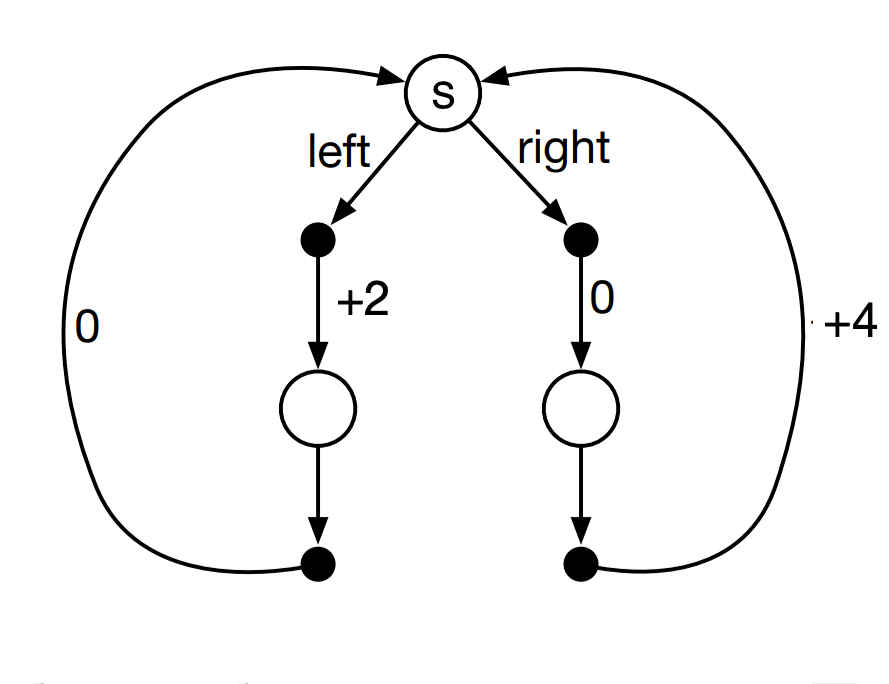
\includegraphics[width=0.6\linewidth]{figures/figure_3dot22.png}
\end{figure}
\bigspace